\section{The SecureFlow module}\label{sec:flow}
Software usually manipulates information with different security policies. For example, passwords are sensitive data, while names or birth dates are not. During execution sometimes we want to be sure sensitive information don't flow to insecure or public output channels. On the other hand, usually we perform some operations on these reserved data. After a successful login the user is sure the provided password is correct. \\
The goal with \texttt{SecureFlow} is to ensure information flow security and declassification policies at compile-time, so that if a code is correctly compiled there are no certain security violations. \\
\citeauthor{russo2008library} \cite{russo2008library} have developed a monadic approach, but their intensive use of the \texttt{IO} monad makes their solution not fully static.

\subsection{Security lattice}
\texttt{SecureFlow} is based on a lattice structure, first introduced by \citeauthor{denning1976lattice} \cite{denning1976lattice}, and represented in this library as a type family \cite{kiselyov2010fun}. This approach is based on a ticketing system. Listing~\ref{lst:lattice} shows the \texttt{Lattice} module. 
\begin{lstlisting}[caption={The Lattice module}, label={lst:lattice}, breaklines=true]
module Security.Lattice (LEQ, Ticket(Ticket)) where

type family LEQ sl sh :: Constraint
data Ticket s = Ticket
\end{lstlisting}
Basically, \texttt{LEQ}, as a type family, represents a partial function at the type level. Applying the function to parameters (called \textit{type indices}) yields a type. Type families permit a program to compute what data constructors it will operate on, rather than having them fixed statically. Here, LEQ means \textit{Less or Equal}. Trusted programmers are asked to instantiate it specifying the real security lattice. A three level lattice example is shown in Listing~\ref{lst:3lvs}.
\begin{lstlisting}[caption={Three levels lattice}, label={lst:3lvs}, breaklines=true]
module ThreeLevels (Low, Medium, High, low, medium) where

data Low    = L
data Medium = M
data High   = H

type instance (LEQ Low Low)       = ()
type instance (LEQ Low Medium)    = ()
type instance (LEQ Low High)      = ()
type instance (LEQ Medium Medium) = ()
type instance (LEQ Medium High)   = ()
type instance (LEQ High High)     = ()

low :: Ticket Low
low = Ticket

medium :: Ticket Medium
medium = Ticket

high :: Ticket High
high = Ticket
\end{lstlisting}
Here, \texttt{Low}, \texttt{Medium} and \texttt{High} are singleton types (\cite{stone2000singleton}, \cite{pierce2005advanced}). Basically, singleton types are those which have only one value. Thus, the value of a singleton type has a unique type representing the value. A type theory that allows types to be parameterised by values (like the one adopted by Haskell) can use singleton types to let types depend on singleton values. The sequence of \texttt{type instance} allows programmers to specify the relations among \texttt{Low}, \texttt{Medium} and \texttt{High}. Listing~\ref{lst:3lvs} shows also a ticketing system instance. Tickets are generally used as a level proof. Note that the \texttt{high} ticket is not exported, so that one may get access to high secure data only according to the declassification policies. \\

\subsection{SecureFlow Implementation}
Basically, \texttt{SecureFlow} is just an identity monad instance tagged with a proposition allowing access to its value. Actually, that proposition is just a ticket. Listing~\ref{lst:secureflow} shows the module.
\begin{lstlisting}[caption={SecureFlow monad}, label={lst:secureflow}, breaklines=true]
data SecureFlow s a = Allowed a | Denied
type Hatch s a b = SecureFlow s (a -> Maybe b)

instance Functor (SecureFlow s) where
  fmap f (Allowed x)  = Allowed $ f x
  fmap _ Denied       = Denied

instance Applicative (SecureFlow s) where
  pure x                      = Allowed x
  (Allowed f) <*> (Allowed x) = Allowed $ f x
  _ <*> _                     = Denied

instance Monad (SecureFlow s) where
  return            = pure
  (Allowed a) >>= f = f a
  Denied >>= _      = Denied
  fail _            = Denied
  
open :: LEQ s s' => Ticket s' -> SecureFlow s a -> Maybe a

up :: LEQ s s' => SecureFlow s a -> SecureFlow s' a

declassifyWith :: (LEQ s k, LEQ s' s) => Hatch k a b -> SecureFlow s a -> SecureFlow s' b
\end{lstlisting}
%\begin{frame}{Functor}
	\begin{itemize}
		\item Values can be encapsulated in contexts
		\item Applying a function yields different results depending on the context
	\end{itemize}
	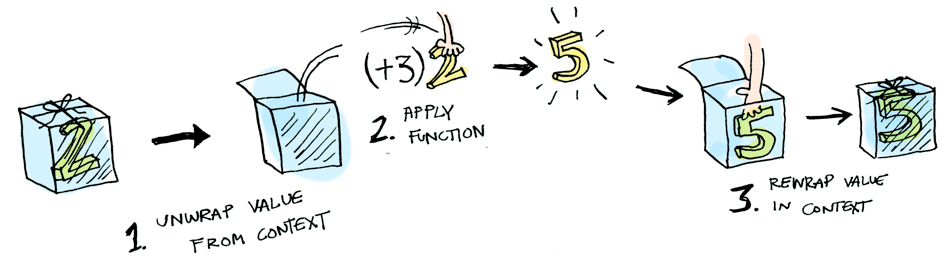
\includegraphics[scale=0.33]{fmap}
	\begin{itemize}
		\item<2-> Generic functions on contexts!
	\end{itemize}
\end{frame}
%\begin{proposition}
\texttt{SecureFlow}, as defined, is an applicative functor.
\end{proposition}
\begin{proof}
We are to prove the four applicative laws.
\begin{enumerate}
	\item \textbf{Identity}: \texttt{pure id <*> v = v}
	\item \textbf{Homomorphism}: \\ \texttt{pure f <*> pure x = pure (f x)}
	\item \textbf{Interchange}: \\ \texttt{u <*> pure y = pure (\$ y) <*> u}
	\item \textbf{Composition}: \texttt{pure (.) <*> u <*> v <*> w = u <*> (v <*> w)}
\end{enumerate}
\end{proof}
\begin{proposition}
\texttt{SecureFlow}, as defined, is a monad.
\end{proposition}
\begin{proof}
We are to prove the three monad laws. 
\begin{enumerate}
	\item \textbf{Left identity}: \texttt{return a >>= f = f a}
		\begin{lstlisting}
(return a >>= f) = (pure a >>= f) = 
= ((Allowed a) >>= f) = f a
		\end{lstlisting}
	
	\item \textbf{Right identity}: \texttt{m >>= return = m}
		\begin{enumerate}
			\item \texttt{m = Allowed a}:
			\begin{lstlisting}
((Allowed a) >>= return) = 
= (return a) = (pure a) = 
= (Allowed a) = m
			\end{lstlisting}
			\item \texttt{m = Denied}:
			\begin{lstlisting}
(Denied >>= return) = Denied = m
			\end{lstlisting}
		\end{enumerate}
	
	\item \textbf{Associativity}: \texttt{(m >>= f) >>= g = m >>= ($\backslash$x -> f x >>= g)} 
		\begin{enumerate}
			\item \texttt{m = Allowed a}:
			\begin{lstlisting}
(((Allowed a) >>= f) >>= g) = 
= ((f a) >>= g) = (g (f a))

(Allowed a >>= (\x -> f x >>= g)) =
= (\x -> f x >>= g) a = 
= ((f a) >>= g) = (g (f a))
			\end{lstlisting}
			\item \texttt{m = Denied}:
			\begin{lstlisting}
((Denied >>= f) >>= g) = 
(Denied >>= g) = Denied =
(Denied >>= (\x -> f x >>= g))
			\end{lstlisting}
		\end{enumerate}
\end{enumerate}
\texttt{SecureFlow} satisfies the three monad laws, hence it is a monad.
\end{proof}
\texttt{SecureFlow} is, obviously, also a functor and an applicative. The proof is largely similar to the last one, so it is omitted.